%Thema ist immer noch LTE
\subsection{Channels}
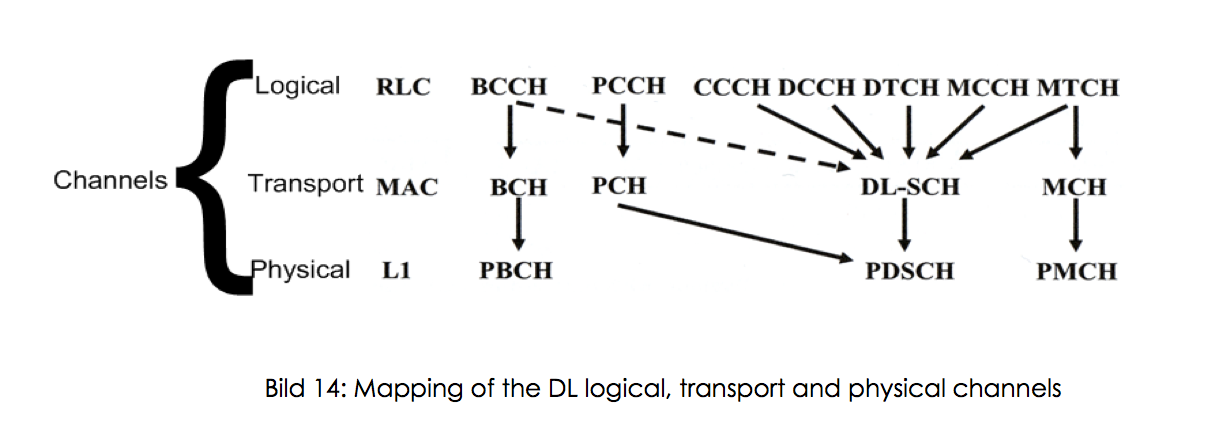
\includegraphics[width = 0.8 \linewidth]{./Pics/Ch1.png}
\subsubsection{Logische Kanäle im UL und DL}
\textbf{CCCH : Common Control Channel: } \\
Transportiert Kontrollinformationen zwischen UEs und dem Netzwerk. Wird verwendet, wenn UEs keine RRC Verbindung mit dem Netzwerk haben \\
\textbf{DCCH : Dedicated Control Channel: } \\
Point to Point und bidirektionaler (UL und DL) Kanal für bestimmte Kontrollinformationen zwischen UE und dem Netzwerk. Wird für UEs verwendet, welche eine RCC Verbindung haben. \\
\textbf{DTCH : Dedicated Traffic Channel: } \\
Point-to-Point Kanal, der einem UE zugewiesen ist für das Senden von Userdaten UP. UL oder DL Richtung. \\
\subsubsection{Logische Kanäle im DL}
\textbf{BCCH Broadcast Control Channel: } \\
Ein DL Kanal um Systemkontroll-Informationen an alle UEs in Reichweite zu senden. \\
\textbf{PCCH Paging Control Channel: } \\
Dieser Kanal wird verwendet um ein UE zu finden, wenn der Aufenthaltsort nicht genau bekannt ist (Paging). \\
\textbf{MCCH Multicast Control Channel: } \\
Point-to-Multipoint Kanal um Multimedia Broadcast Multicast Services (MBMS) Kontrollinformationen vom Netzwerk zum UE zu senden. Die Informationen können einen oder mehrere MTCH betreffen. Dieser Kanal wird nur von UEs benutzt, die MBMS empfangen. \\
\textbf{MTCH Multicast Traffic Channel: } \\
Point-to-Multipoint Kanal um Multicast Daten vom Netzwerk zu den UEs zu senden. Kanal wird nur von UEs benutzt, die MBMS empfangen. \\
\subsubsection{Transport Kanäle im DL}
\textbf{BCH Broadcast Channel: } \\
Sendet Systeminformationen innerhalb der ganzen Zelle. \\
\textbf{PCH Paging Channel: } \\
Sendet Paging Nachrichten innerhalb der ganzen Zelle. \\
\textbf{DL-SCH Downlink Shared Channel: } \\
Unterstütz dynamische Verbindungsanpassung mit unterschiedlichen Sendeleistungen, unterschiedlichen Modulationsarten, unterschiedlichen Codierungen. Unterstützt Hybrid Automatic Repeat Request (HARQ). Unterstützt MBMS. \\
\textbf{MCH Multicast Channel: } \\
Sendet NAchrichten innerhalb der ganzen Zelle. Unterstützt MBMS Single Frequency Network (MBSFN). Dies ist die Kombination von einer MBMS Übertragung über mehrere Zellen hinweg. \\
\subsubsection{Physikalische Kanäle im DL}
\textbf{PBCH Physical Broadcast Channel: } \\
Unterstützt die QPSK Modulationsart. \\
\textbf{PDSCH Physical Downlink Shared Channel: } \\
Überträgt den DL-SCH und den PCH. Unterstützt die folgenden Modulationsarten: QPSK, 16-QAM, und 64-QAM. \\
\textbf{PMCH Physical Multicast Channel: } \\
Überträg den MCH. Unterstützt die folgenden Modulationsarten: 16-QAM und 64 QAM. \\ \\
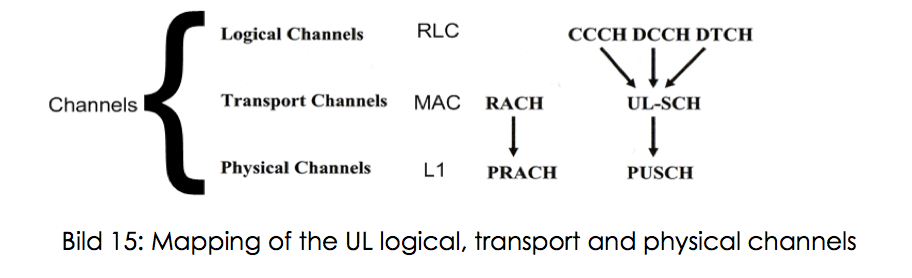
\includegraphics[width = 0.7 \linewidth]{./Pics/Ch2.png}
\subsubsection{Transportkanäle im UL}
\textbf{RACH Random Access Channel: } \\
Hier kann es zu Kollisionen kommen. Kanal wird bei einem Erstkontakt verwendet, wenn noch keine Timing-Information vorhanden sind. \\
\textbf{UL-SCH Uplink Shared Channel: } \\
Unterstützt dynamische Verbindungsanpassung mit unterschiedlichen Sendeleistungen, unterschiedlichen Modulationsarten, unterschiedlichen Codierungen. Unterstützt Hybrid ARQ.\\
\subsubsection{Physikalische Kanäle im UL}
\textbf{PRACH Physical Random Access Channel: } \\
Überträgt die random access Preambel. \\
\textbf{PUSCH Physical Uplink Shard Channel: } \\
Überträgt den UL-SCH. Unterstützt die folgenden Modulationsarten: QPSK, 16-QAM und 64-QAM. \\
\subsubsection{Scheduling: eine Aufgabe des eNodeB}
Durch zentrales durch das Netzwerk geregeltes Scheduling ermöglicht eine schnelle Reaktion auf veränderte Bedingungen an der Luftschnittstelle, das QoS übwerachen und steuern, kontrolle von Überlastsituationen sowie optimaler Durchsatz bei ca 10 \% Fehler. \\
Im Downlink ist es nur solange trivial, wie nur ein Benutzer in der Zelle ist, sonst müssen Entscheidungen welche Daten pro Subframe und Bearer gesendet werden. Es muss das QoS sicher gestellt werden und bei gleicher Priorität andere Faktoren beachtet werden, wie Radiobedingungen und Proportioal Fair Scheduler. \\
Im Uplink sendet das UE einen Schedule Request an den eNodeB. Ressourcen werden dann über PDCCH zugeteilt. Eine weitere Kontrollmöglichkeit ist das versenden von Buffer Status Reports. Die Sendeleistung im UE hat Einfluss auf die Modulationsart, das Codierungsverfahren sowie die Resource Blocks. \\
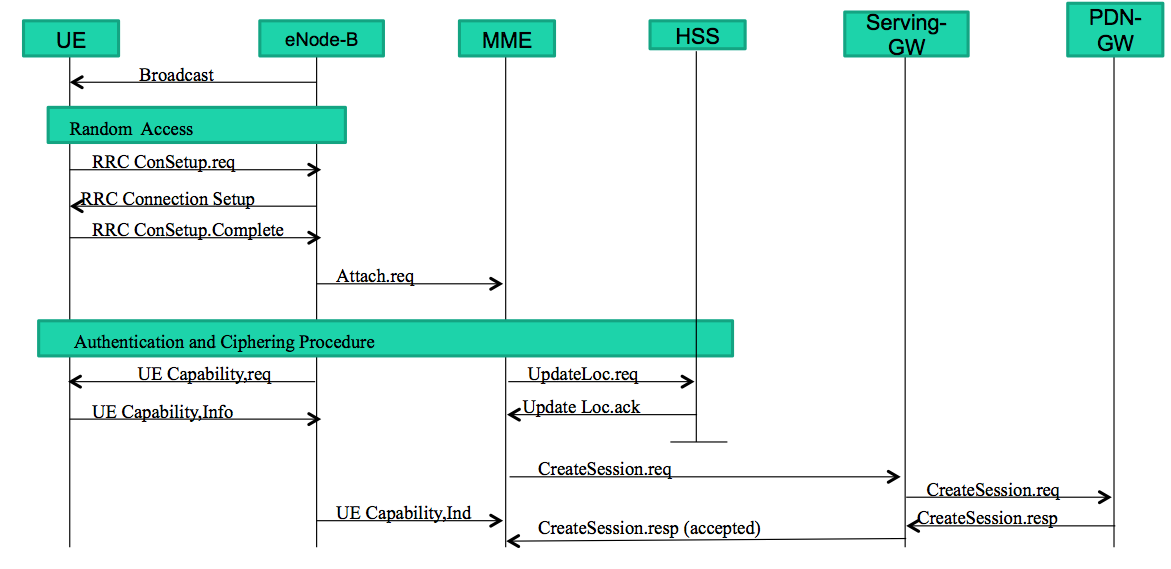
\includegraphics[width = 0.8 \linewidth]{./Pics/db1.png}\\
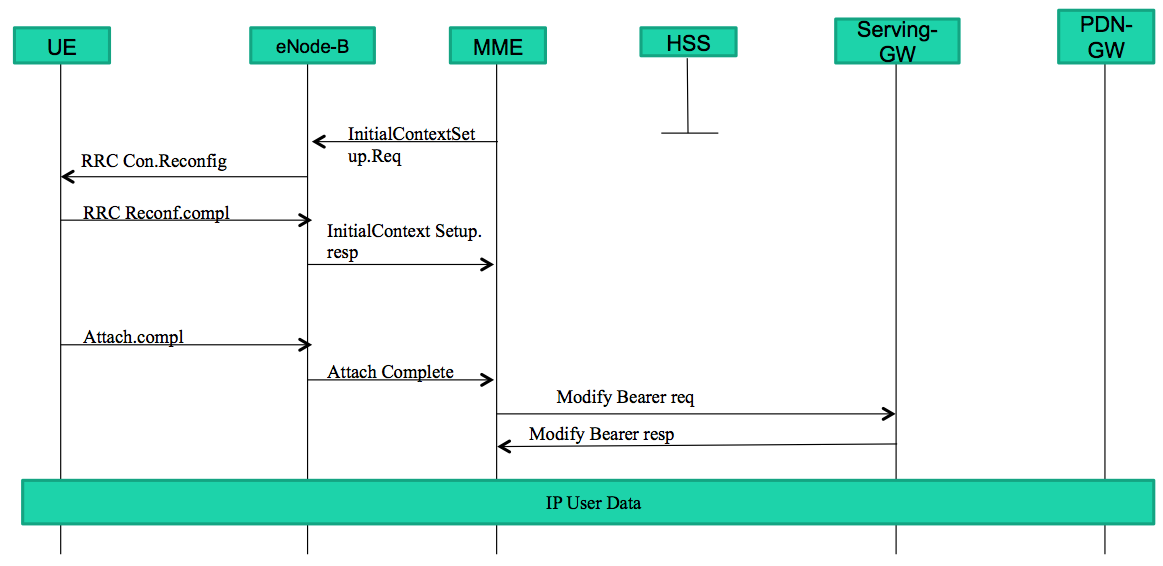
\includegraphics[width = 0.8 \linewidth]{./Pics/db2.png}
\subsection{Mobility}
Die Mobilitätsprozeduren für angemeldete (attached) UEs können in zwei Modes eingeteilt werden, den idle Mode sowie den connected Mode.
\subsubsection{Idle Mode}
Im idle Mode erfolgt die Zellauswahl (Cell selection, reselection) durch die UE. Die UE misst die einkommenden Signale und entscheidet dann selbständig welche Zelle sie momentan angehört. Die UE kontrolliert die Auswahl mittels Parameter in den broadcast Meldungen.
\subsubsection{Connected Mode}
Hier gibt das Netzwerk den Zeitpunkt sowie die nächste Zelle vor, bei einem Handover. Auch diese Auswahl basiert auf den Messungen des UE.

\subsubsection{MME Mobility Management Entity}
Die EPS (Envolved Packet System) Komponente Mobility Management Entity (MME) ist die zentrale Komponente des Mobility Managements. Die MME bedient nur Control Plane (CP) Daten, keine User Plane (UP) Daten. Zudem hat das MME eine Anbindung an den HSS (Home Subscriber Server), in welchem alle Subscriberdaten gespeichert werden. \\
Der MME hat mehrer Funktionen, zum einen ist er für die Authentication und die Security verantwortlich und zum anderen für das Mobility Management. Die Authentication wird durch Challenge/Response realisiert. Danach werden Ciphering Keys für das UP und das CP berechnet.\\
Im Mobility Management initialisiert das MME das Paging in einer Tracking Area (TA), wenn Daten für ein UE ankommen, welches sich im idle Mode befindet. Die MME wird von den UEs (idle und connected), welche sich in der Service Area der MME befinden, über den Aufenthaltsort informiert und dann benachrichtigt das MME deren HSS über den Aufenthaltsort der UEs. Das MME ist zudem für die kontrolle des Auf-, Abbaus und die Modifizierung der Bearer zuständig. Zudem organisiert es das Tunnel switching bei HO. \\
